\input{preamble.tex}

\title{Отчет по лабораторной работе № 3. \\ Анализ трафика в Wireshark}
\author{Данила Стариков \\ НПИбд-02-22}
\date{2024}

\begin{document}

\maketitle
\newpage

\tableofcontents

\newpage
\section{Цель работы}
Изучение посредством Wireshark кадров Ethernet, анализ PDU протоколов транспортного и прикладного уровней стека TCP/IP.
\newpage
\section{Выполнение работы}

\subsection{MAC-адресация}
\begin{enumerate}
    \item С помощью команды ifconfig вывели информацию о текущем сетевом соединении (Рис. \ref{01}):
    % Прокомментировать
\item MAC-адреса сетевых интерфейсов на компьютере (Рис. \ref{01}):
    \begin{itemize}
        \item MAC-адрес wlp2s0 - a2:19:64:3c:02:6b.
        \item MAC-адрес enp1s0 - 80:e8:2c:1d:41:0a.
    \end{itemize}

\item Описание структуры MAC-адресов вашего устройства (Рис. \ref{01}):
    \begin{itemize}
        \item MAC-адрес wlp2s0 - a2:19:64:3c:02:6b. Адрес является индивидуальным и локально администируемым, что определяется двумя младшими битами первого октета: \(a2_{16} = 10100010_2\).
        \item MAC-адрес enp1s0 - 80:e8:2c:1d:41:0a. Адрес является индивидуальным и глобально администриуемым (\(80_{16} = 10000000_2\)).
    \end{itemize}

\begin{center}
    \centering
    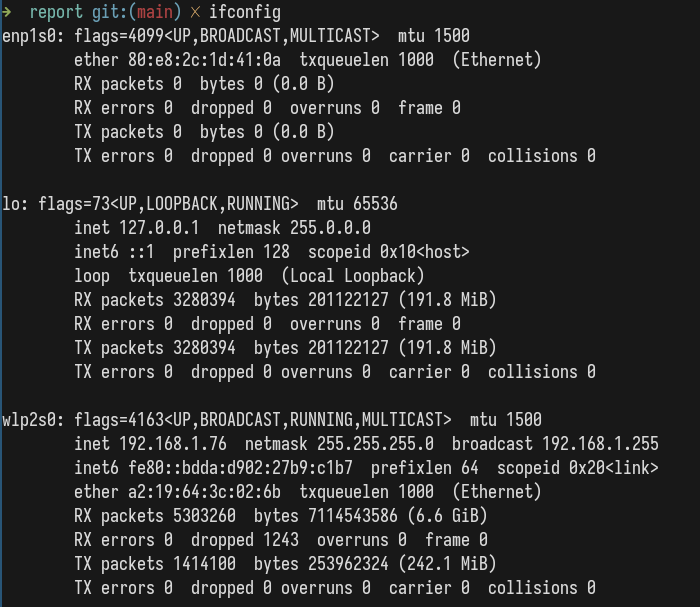
\includegraphics[width=\textwidth]{../images/image01.png}
    \captionof{figure}{Вывод команды ifconfig.}
    \label{01}
\end{center}

\end{enumerate}

\subsection{Анализ кадров канального уровня в Wireshark}
\begin{enumerate}
\item Установили на вашем устройстве Wireshark.
    \begin{minted}{bash}
sudo dnf install wireshark
    \end{minted}
\item Настроили административные права для захвата пакетов (Рис. \ref{06}):
    \begin{minted}{bash}
sudo -i
groupadd wireshark
gpasswd -a dastarikov wireshark
chgrp wireshark /usr/bin/dumpcap
chmod 750 /usr/bin/dumpcap
setcap cap_net_raw,cap_net_admin=eip /usr/bin/dumpcap
    \end{minted}
Затем в основном пользователе добавили себя в группу wireshark: {\tt newgrp wireshark}.

\begin{center}
    \centering
    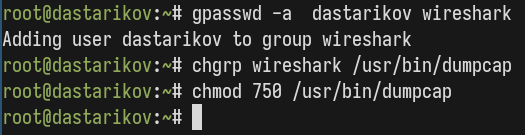
\includegraphics[width=\textwidth]{../images/image06.png}
    \captionof{figure}{Настройка административных прав для захвата пакетов.}
    \label{06}
\end{center}

\item Запустили Wireshark. Выбрали активный на вашем устройстве сетевой интерфейс. Убедились, что начался процесс захвата трафика (Рис. \ref{10}).

\begin{center}
    \centering
    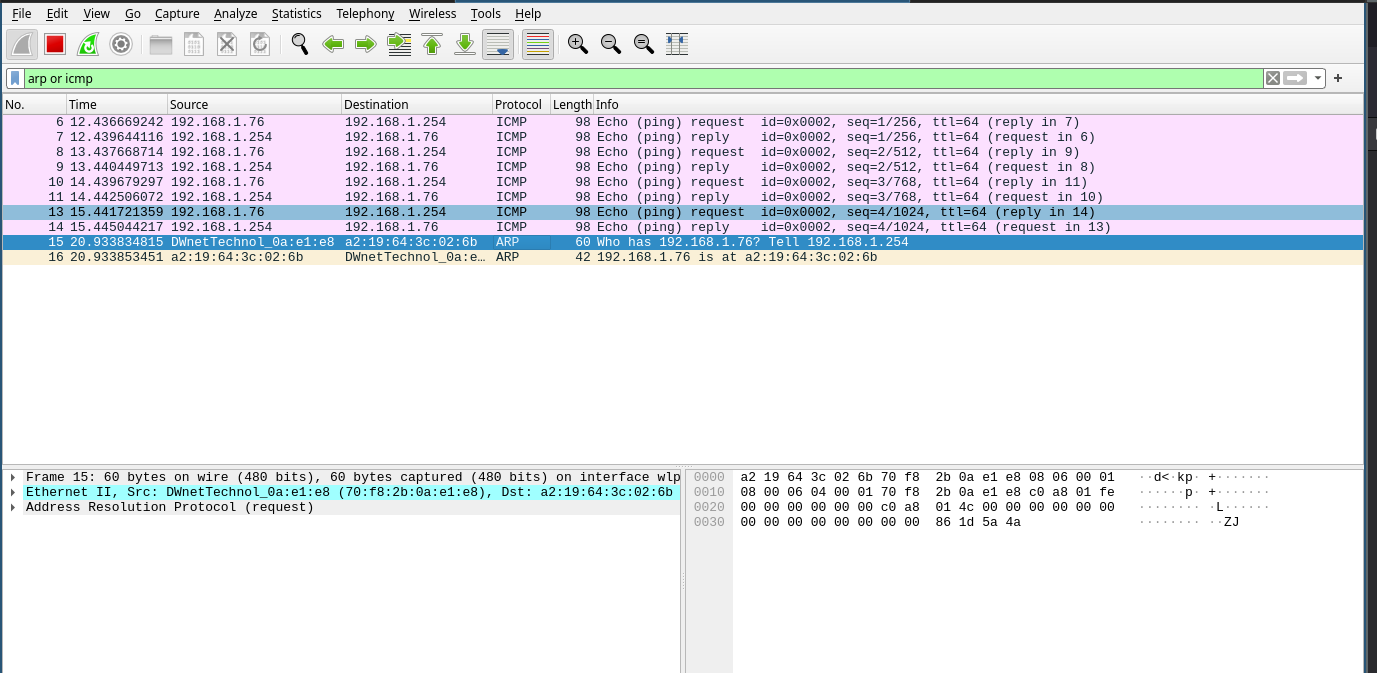
\includegraphics[width=\textwidth]{../images/image10.png}
    \captionof{figure}{Интерфейс Wireshark.}
    \label{10}
\end{center}

\item На устройстве в консоли определили с помощью команды {\tt ifconfig} IP-адрес устройства и шлюз по умолчанию (default gateway) (Рис. \ref{07}).

\begin{center}
    \centering
    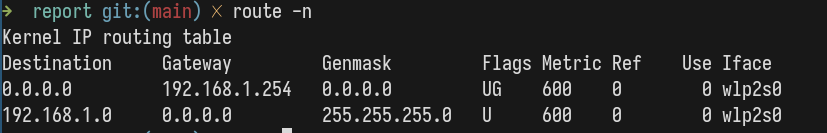
\includegraphics[width=\textwidth]{../images/image07.png}
    \captionof{figure}{Определение IP-адреса шлюза.}
    \label{07}
\end{center}

\item На устройстве в консоли с помощью команды {\tt ping 192.168.1.254} пропинговали шлюз по умолчанию (Рис. \ref{08}).

\begin{center}
    \centering
    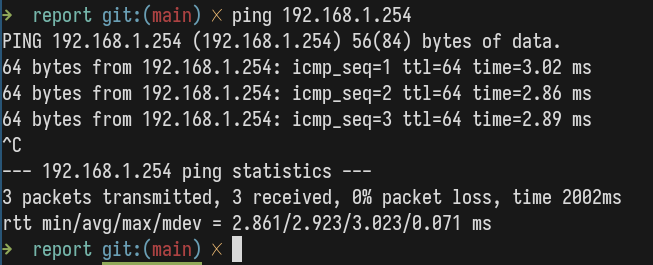
\includegraphics[width=\textwidth]{../images/image08.png}
    \captionof{figure}{Пингование шлюза.}
    \label{08}
\end{center}

\item В Wireshark остановили захват трафика. В строке фильтра пропишите фильтр {\tt arp or icmp} (Рис. \ref{10}).
\item Изучили эхо-запрос и эхо-ответ ICMP в программе Wireshark:

    \begin{itemize}
\item На панели списка пакетов (верхний раздел) выбрали первый указанный кадр ICMP — эхо-запрос. Изучили информацию на панели сведений о пакете в средней части экрана (Рис. \ref{11}).
    \begin{itemize}
        \item Длина кадра - 98 байтов
        \item Тип Ethernet - IPv4
        \item Mac-адрес источника - a2:19:64:3c:02:6b
        \item Mac-адрес шлюза - 70:f8:2b:0a:e1:e8
    \end{itemize}

\begin{center}
    \centering
    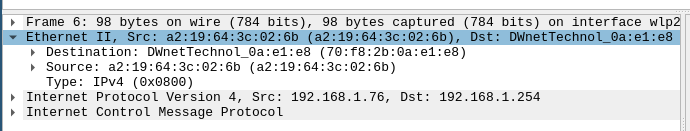
\includegraphics[width=\textwidth]{../images/image11.png}
    \captionof{figure}{Информация об эхо-запросе.}
    \label{11}
\end{center}

    В отчёте укажите длину кадра, к какому типу Ethernet относится кадр, определите MAC-адреса источника и шлюза, определите тип MAC-адресов.
\item На панели списка пакетов (верхний раздел) выбрали второй указанный кадр ICMP — эхо-ответ. Изучите информацию на панели сведений о пакете в средней части экрана (Рис. \ref{12}).
    \begin{itemize}
        \item Длина кадра - 98 байтов
        \item Тип Ethernet - IPv4
        \item Mac-адрес источника - 70:f8:2b:0a:e1:e8
        \item Mac-адрес шлюза - a2:19:64:3c:02:6b
    \end{itemize}

\begin{center}
    \centering
    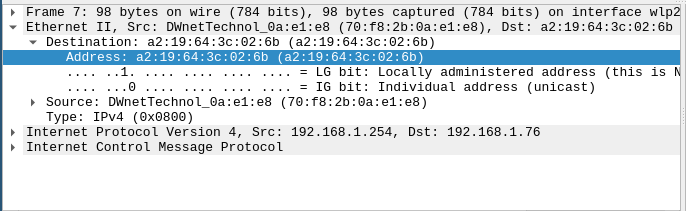
\includegraphics[width=\textwidth]{../images/image12.png}
    \captionof{figure}{Информация об эхо-ответе.}
    \label{12}
\end{center}

    \end{itemize}
\item Изучили кадры данных протокола ARP. Изучили данные в полях заголовка Ethernet II (Рис. \ref{13}).

\begin{center}
    \centering
    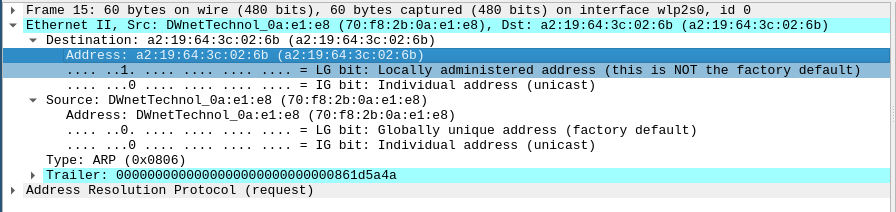
\includegraphics[width=\textwidth]{../images/image13.png}
    \captionof{figure}{Информация кадра протокола ARP.}
    \label{13}
\end{center}

\item Начали новый процесс захвата трафика в Wireshark (Рис. \ref{15}). На устройстве в консоли пропинговали известный адрес, {\tt ping google.com}.
\item В Wireshark остановили захват трафика. Изучили запросы и ответы протоколов ARP и ICMP. Определили MAC-адреса источника и получателя, определили тип MAC-адресов.

\begin{center}
    \centering
    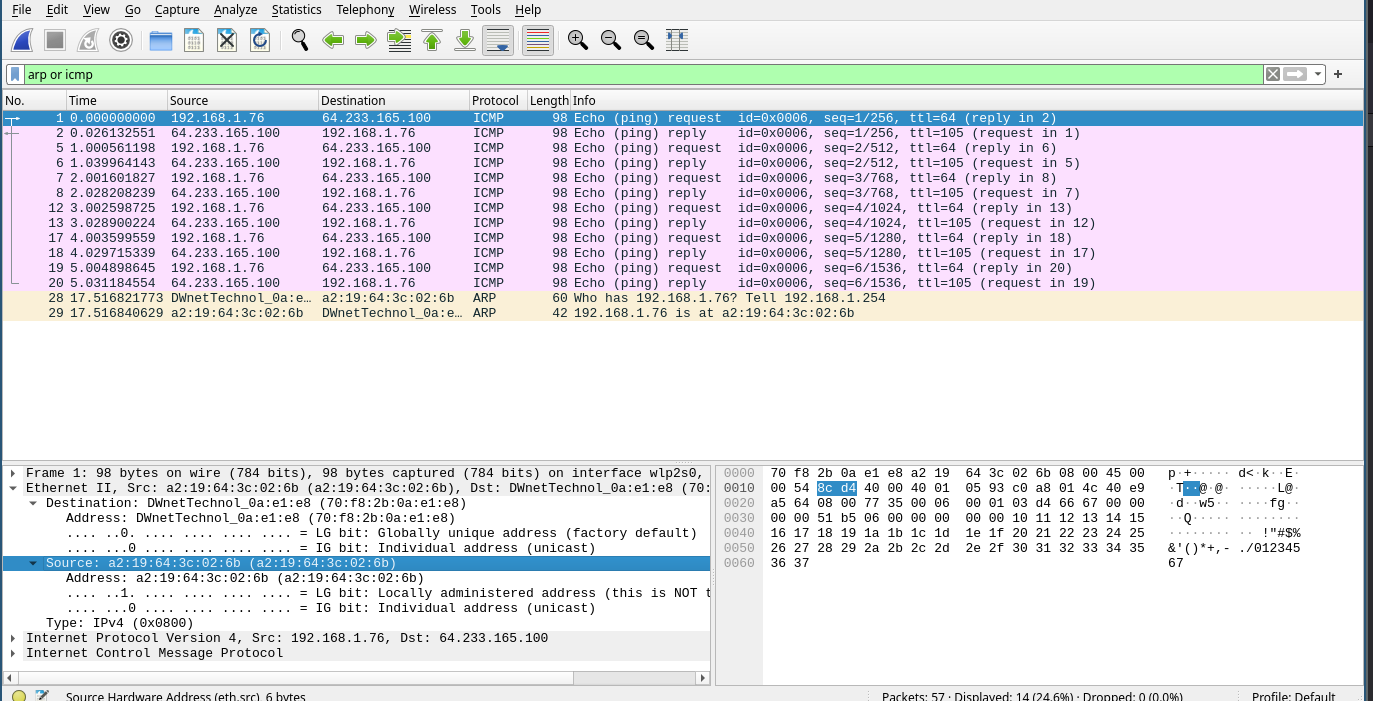
\includegraphics[width=\textwidth]{../images/image15.png}
    \captionof{figure}{Изучение трафика между устройством и google.com.}
    \label{15}
\end{center}

Данные эхо-запроса (Рис. \ref{16}):
\begin{itemize}
        \item длина кадра - 98
        \item тип ethernet - ipv4
        \item mac-адрес источника - a2:19:64:3c:02:6b
        \item mac-адрес получателя - 70:f8:2b:0a:e1:e8
\end{itemize}


\begin{center}
    \centering
    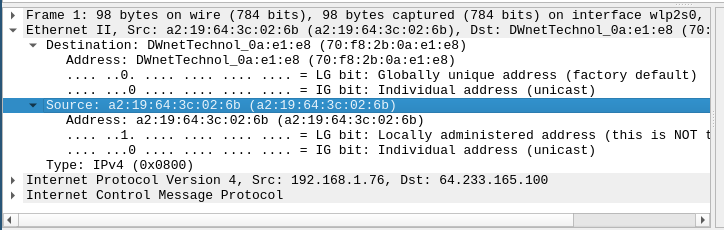
\includegraphics[width=\textwidth]{../images/image16.png}
    \captionof{figure}{Эхо-запрос к google.com}
    \label{16}
\end{center}

Данные эхо-ответа (Рис. \ref{17}):
\begin{itemize}
        \item длина кадра - 98
        \item тип ethernet - ipv4
        \item mac-адрес источника - 70:f8:2b:0a:e1:e8
        \item mac-адрес получателя - a2:19:64:3c:02:6b
\end{itemize}

\begin{center}
    \centering
    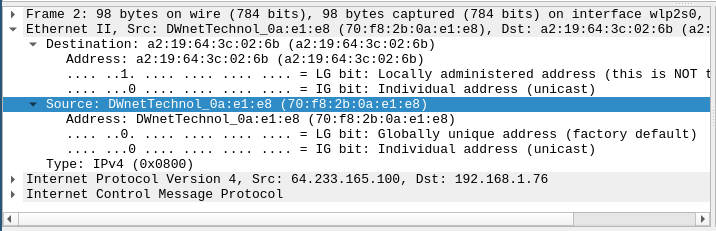
\includegraphics[width=\textwidth]{../images/image17.png}
    \captionof{figure}{Эхо-ответ от google.com}
    \label{17}
\end{center}

\end{enumerate}

\subsection{Анализ протоколов транспортного уровня в Wireshark}
\begin{enumerate}
\item Запустили Wireshark. Выбрали активный сетевой интерфейс и убедились, что начался процесс захвата трафика.
\item На устройстве в браузере перешли на сайт, работающий по протоколу HTTP (например, на сайт CERN \url{http://info.cern.ch/}).

\item В Wireshark в строке фильтра указали http и проанализировали информацию по протоколу TCP в случае запросов и ответов (Рис. \ref{18}).

Кадры по протоколу HTTP уже больше (432, 932, 401 и т.д. Кб), в поле MAC-адрес получателя также определен MAC-адрес шлюза.

\begin{center}
    \centering
    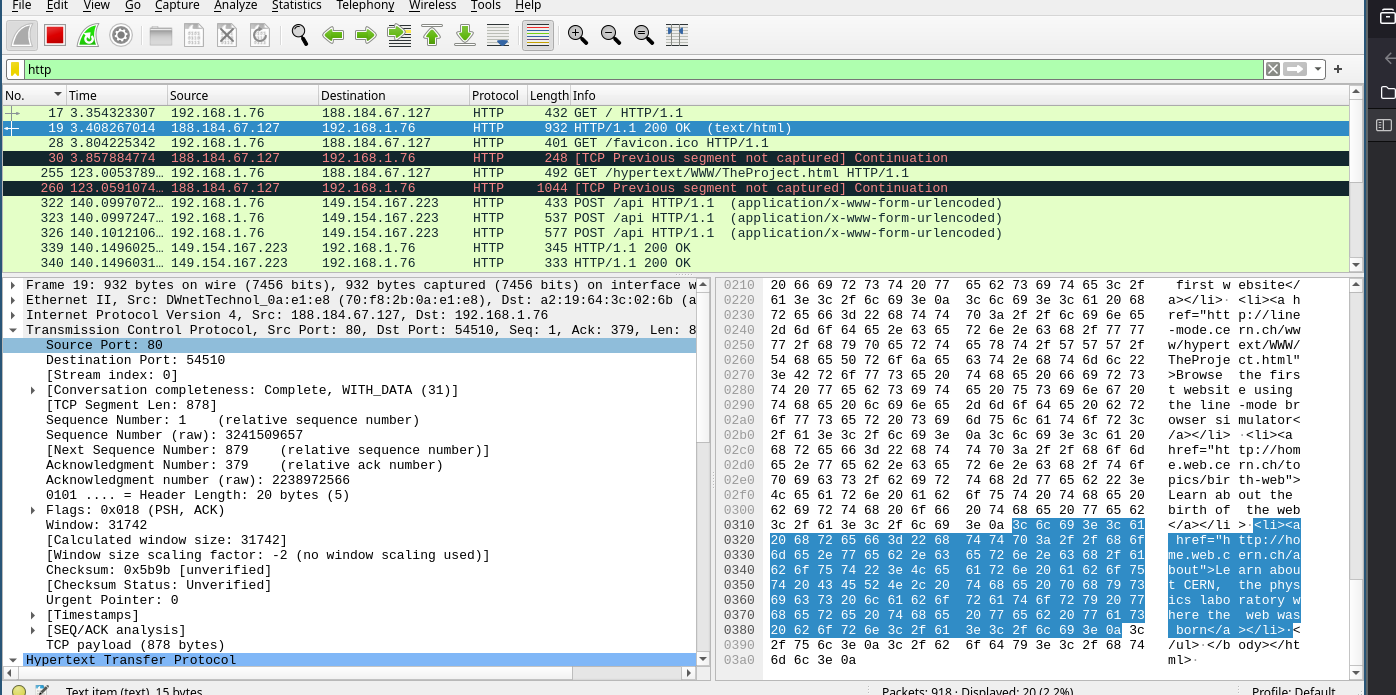
\includegraphics[width=\textwidth]{../images/image18.png}
    \captionof{figure}{Фильтрование трафика по протоколу HTTP.}
    \label{18}
\end{center}

\item Wireshark в строке фильтра указали dns и проанализировали информацию по протоколу UDP в случае запросов и ответов (Рис. \ref{19}). Кадры меньше, чем в HTTP (83, 83, 123 и т.д. Кб), информация о отправителе и получателе такая же.

\begin{center}
    \centering
    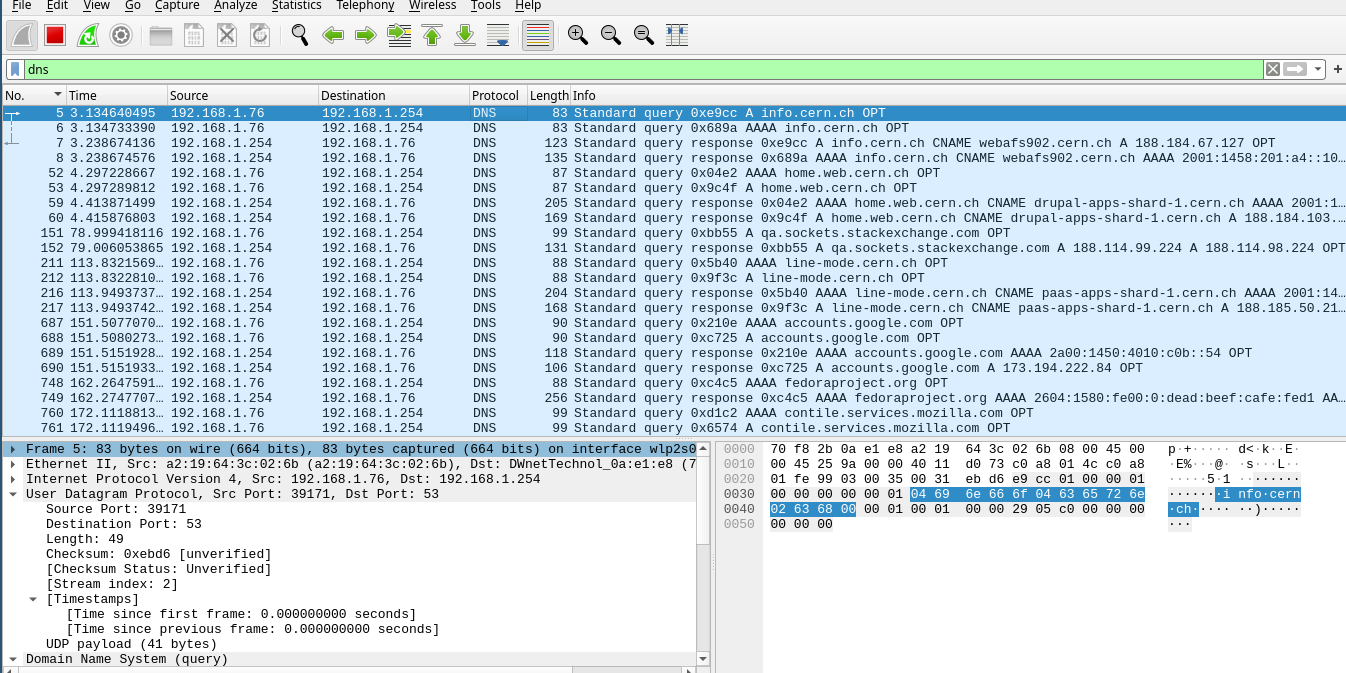
\includegraphics[width=\textwidth]{../images/image19.png}
    \captionof{figure}{Фильтрование трафика по протоколу UDP.}
    \label{19}
\end{center}

\item Wireshark в строке фильтра указали quic и проанализировали информацию по протоколу quic в случае запросов и ответов (Рис. \ref{24}). В пакете QUIC задан большой размер, хотя иногда последний блок пакета может быть нулевым.

\begin{center}
    \centering
    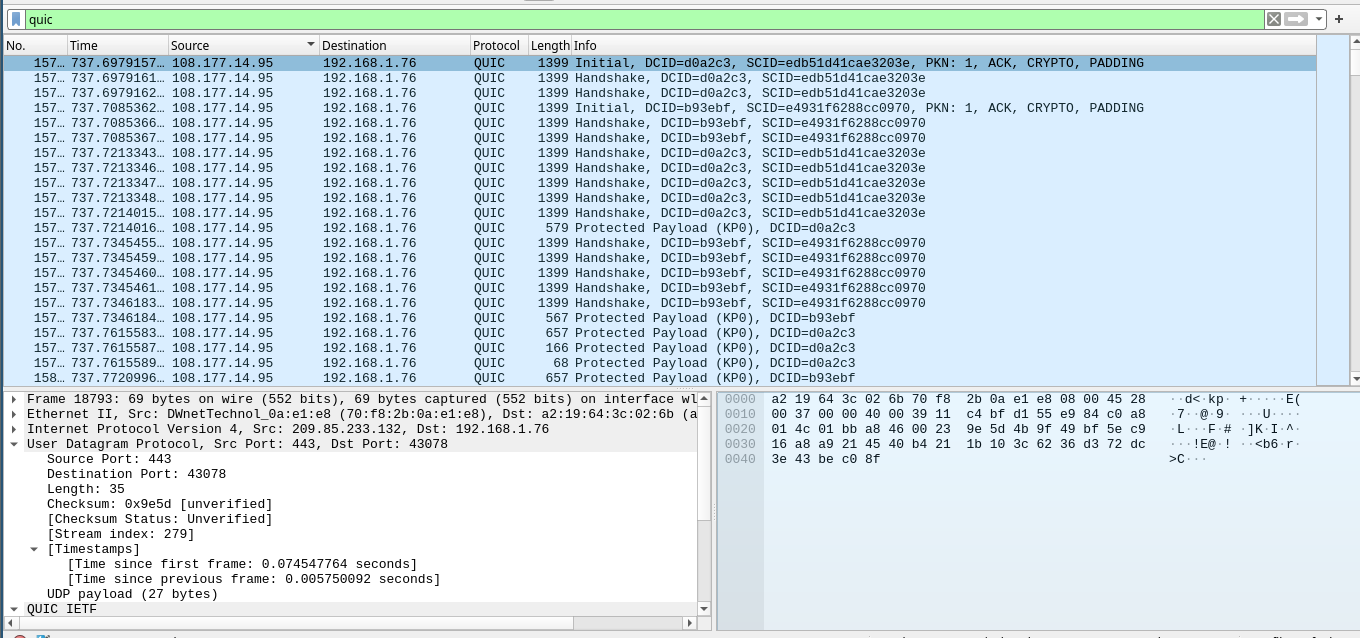
\includegraphics[width=\textwidth]{../images/image24.png}
    \captionof{figure}{Фильтрование трафика по протоколу QUIC.}
    \label{24}
\end{center}

\item Остановили захват трафика в Wireshark.
\end{enumerate}
\subsection{Анализ handshake протокола TCP в Wireshark}
\begin{enumerate}
\item Запустили Wireshark. Выбрали активный сетевой интерфейс и убедились, что начался процесс захвата трафика.
\item На устройстве соединились по HTTP с сайтом для захвата в Wireshark пакетов TCP.
\item В Wireshark проанализировали handshake протокола TCP, в отчёте приведите пример с пояснениями изменения значений соответствующих сообщений при установлении соединения по TCP (Рис. \ref{22}). Для установления соединения по TCP используется процесс three-way handshake или трехстороннее рукопожатие. Происходит обмен тремя пакетами:
    \begin{enumerate}
        \item Клиент отправляет сегмент с установленным флагом SYN.
        \item Сервер получает запрос и отправляет ответный сегмент с одновременно установленными флагами SYN+ACK. Также увеличивается на 1 параметр Acknoledgement number
        \item После получения клиентом сегмента с флагами SYN+ACK соединение считается установленным, клиент, в свою очередь, отправляет в ответ сегмент с флагом ACK, обновленными номерами последовательности, и не содержащий полезной нагрузки.
    \end{enumerate}

\begin{center}
    \centering
    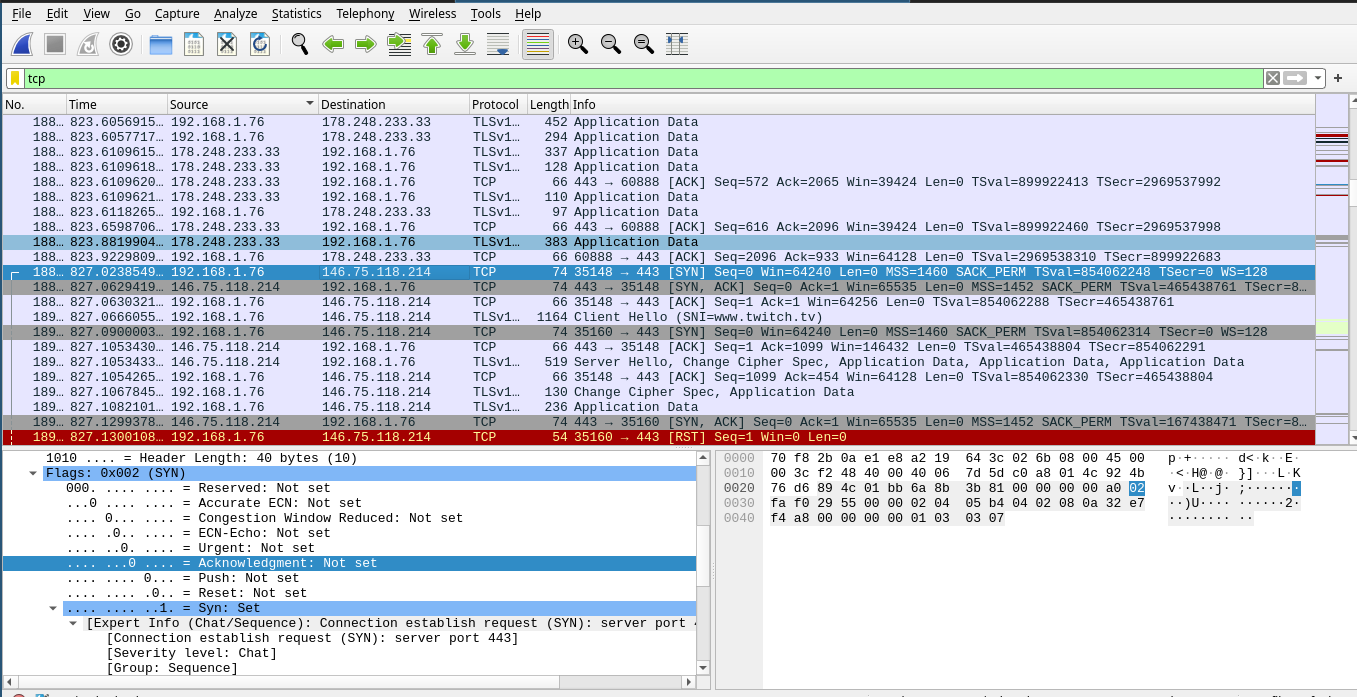
\includegraphics[width=\textwidth]{../images/image22.png}
    \captionof{figure}{handshake протокола TCP.}
    \label{22}
\end{center}

\item В Wireshark в меню «Статистика» выбрали "График Потока" (Рис. \ref{23}). 

\begin{center}
    \centering
    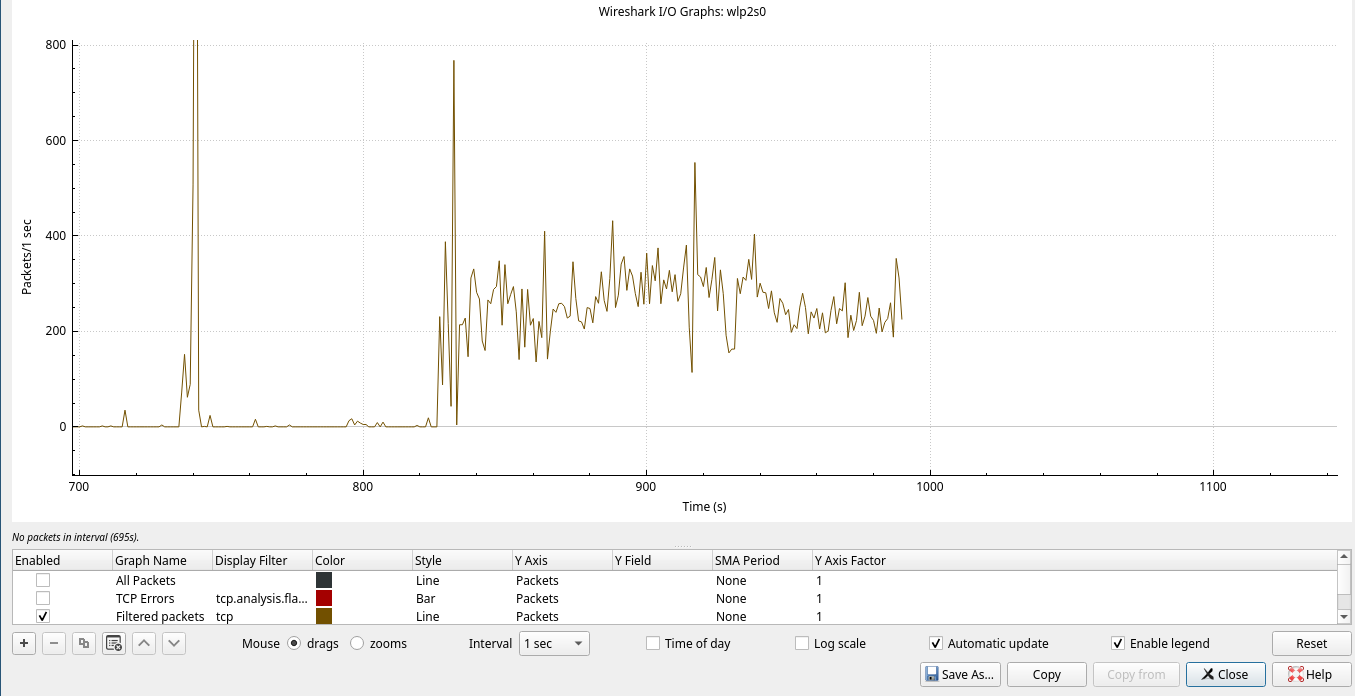
\includegraphics[width=\textwidth]{../images/image23.png}
    \captionof{figure}{График потока TCP пакетов.}
    \label{23}
\end{center}

\item Остановили захват трафика в Wireshark.
\end{enumerate}

\section{Выводы}
В процессе выполнения лабораторной работы научились работать с программой Wireshark для анализа различных сетевых пакетов на транспортном и прикладном уровнях.
\end{document}
